% CVPR 2023 Paper Template
% based on the CVPR template provided by Ming-Ming Cheng (https://github.com/MCG-NKU/CVPR_Template)
% modified and extended by Stefan Roth (stefan.roth@NOSPAMtu-darmstadt.de)

\documentclass[12pt,twocolumn,letterpaper]{article}

%%%%%%%%% PAPER TYPE  - PLEASE UPDATE FOR FINAL VERSION
% \usepackage[review]{cvpr}      % To produce the REVIEW version
\usepackage{cvpr}              % To produce the CAMERA-READY version
%\usepackage[pagenumbers]{cvpr} % To force page numbers, e.g. for an arXiv version

% Include other packages here, before hyperref.
\usepackage{graphicx}
\usepackage{amsmath}
\usepackage{amssymb}
\usepackage{booktabs}
\usepackage[none]{hyphenat}
\usepackage{array}

% It is strongly recommended to use hyperref, especially for the review version.
% hyperref with option pagebackref eases the reviewers' job.
% Please disable hyperref *only* if you encounter grave issues, e.g. with the
% file validation for the camera-ready version.
%
% If you comment hyperref and then uncomment it, you should delete
% ReviewTempalte.aux before re-running LaTeX.
% (Or just hit 'q' on the first LaTeX run, let it finish, and you
%  should be clear).
\usepackage[pagebackref,breaklinks,colorlinks]{hyperref}

% Support for easy cross-referencing
\usepackage[capitalize]{cleveref}
\crefname{section}{Sec.}{Secs.}
\Crefname{section}{Section}{Sections}
\Crefname{table}{Table}{Tables}
\crefname{table}{Tab.}{Tabs.}

%%%%%%%%% PAPER ID  - PLEASE UPDATE
\def\cvprPaperID{*****} % *** Enter the CVPR Paper ID here
\def\confName{CVPR}
\def\confYear{2023}

\begin{document}

% <><><><><><><><><><><><><><><><><><><>
%               TITLE
% <><><><><><><><><><><><><><><><><><><>
\title{SySeVR: A Framework and Larger Pathway for Using Deep Learning to Detect Software Vulnerabilities}

% <><><><><><><><><><><><><><><><><><><>
%              AUTHORS
% <><><><><><><><><><><><><><><><><><><>
\author{
    Carter Yanac\\
    University of Central Florida\\
    Orlando, FL\\
    {\tt\small yanac7562@knights.ucf.edu}
    \and
    Stefan Werleman\\
    University of Central Florida\\
    Orlando, FL\\
    {\tt\small stefanwerleman@knights.ucf.edu}
}
\maketitle

% <><><><><><><><><><><><><><><><><><><>
%           ABSTRACT - Stefan
% <><><><><><><><><><><><><><><><><><><>
\begin{abstract}
    Deep learning has been a catalyst for the latest breakthroughs in recent technological history. It has been 
    used in computer vision, finance, social media, and more. However, the latest development in deep 
    learning has not been under any of these categories. Researchers have developement deep learning 
    frameworks in the cybersecurity sector. More specifically there have been recent developments for 
    for analyzing software vulnerabilities as a primary aid for software engineers that work with sensitive 
    data and systems. This work paper covers a special type of deep learning framework called SySeVR which is 
    detects software vulnerabities in C/C++ code implementation. We are not only going to cover this framework, 
    in detail but we are also going to cover other existing related frameworks and how it enabled more 
    developments in deep learning such as deep representation learning, VulDeBERT, VulDeePecker, and SAVIOR.
\end{abstract}

% <><><><><><><><><><><><><><><><><><><>
%         INTRODUCTION - Stefan
% <><><><><><><><><><><><><><><><><><><>
\section{Introduction}
\label{sec:intro}

\begin{figure}[t]
    \centering
    \fbox{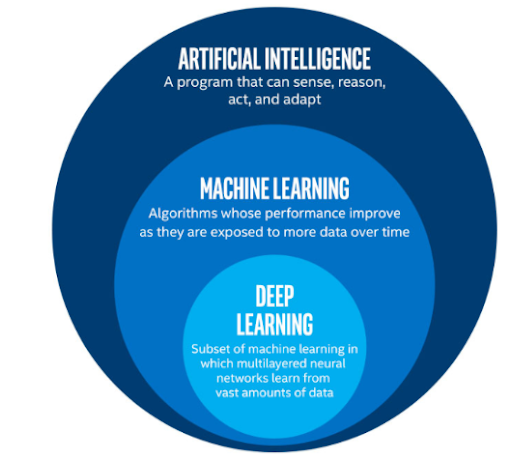
\includegraphics[width=0.47\textwidth]{images/deep_learning/deep_learning_0.png}}

    \caption{Overview of the Artificial Intelligence bubble \cite{Oppermann22}.}
    \label{fig:intro-0}
\end{figure}

More and more companies and organizations are relying on software and automation to become successful. 
Essentially, there is an increasing amount of software that is being pushed to production and this increases 
the number of software vulnerabilities. This gives attackers a bigger playing field for exploiting these 
vulnerabilities which can be catastrophic to many industries so this increases the demand for further improving 
and patching software vulnerabilities. However, with the boom of open-source software community, there an 
abundant amount of code that deep learning (DL) models can learn from in order to detect vulnerable software 
\cite{Lin20}. 

There have been several open-source databases that were created that provides a comprehensive collection of 
software vulnerabilities and defects (Section \ref{sec:data}). This paper is going to cover the different databases that the models 
will use for training and validation. All of the deep learning models in this paper are supervised learning 
models which means they have to learn from some sort of history.

The model that we are going to cover today is the SySeVR framework which is a deep learning model that detects 
software vulnerabilities \cite{Li22}. This will include the datasets it learns from, how its workflow was inspired by 
a computer vision workflow, results, and limitations. Furthermore, this paper is not only going to cover 
SySeVR but it is also going to cover additional frameworks and emphasize the capabilities of deep 
learning for analyzing software. Most importantly, this paper will explain why companies and developers 
should incorporate these existing solutions in the work process so that they push more secure software 
into production and how SySeVR is just one small piece of this puzzle.

% <><><><><><><><><><><><><><><><><><><>
%         DATA - Stefan
% <><><><><><><><><><><><><><><><><><><>
\section{Data}
\label{sec:data}

Databases are extremely important for a wide variety of AI models, especially for deep learning models. 
With the help of the open-source communities organizations were able to create large database for this 
exact purpose.

\subsection{National Vulnerability Database (NVD)}
\label{sub:nvd}

A public repository created by the U.S. government that commonly used for vulnerability management, 
compliance, security measurements, and so on \cite{Nist00}. It has an open-source REST API that can be 
used to provide datasets for deep learning models such as SySeVR to train on (Section \ref{sec:sysevr-framework}).

% <><><><><><><><><><><><><><><><><><><>
%         DEEP LEARNING - Stefan
% <><><><><><><><><><><><><><><><><><><>
\section{Deep Learning (DL)}
\label{sec:deep-learning}

\begin{figure}[t]
    \centering
    \fbox{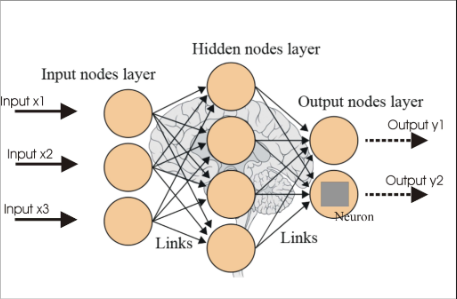
\includegraphics[width=0.47\textwidth]{images/deep_learning/neural_network_0.png}}
    \caption{General architecture of a neural network.}
    \label{fig:dl-0}
\end{figure}

Deep learning (DL) is subset of machine learning that focuses on multi-layered neural networks (NN)
(Figure \ref{fig:intro-0}). Neural networks are inspired by the human brain where the brain learns from 
history or experience and establishes the weights and biases to make decisions. In practice, the neural 
network mimics this exact behavior and is consisted of layers and nodes. NNs can be used for computer vision 
tasks, natural language processing, and pattern recognition.

There are three main layers in an NN: \textbf{input}, \textbf{hidden}, and \textbf{output} layer. 
The input layer of an NN receives the engineered features of a data-point, the outputs of the input layer would
then go through the hidden layer where each node's weight and bias are updated to fit the data-point, and 
then the predictions provided by the output layer (Figure \ref{fig:dl-0}). This is the jist of a 
neural network. However, there are many different types of NNs each of which is tailored for specific 
tasks.

\subsection{Recurrent Neural Network (RNN)}
\label{sub:recurrent-neural-network}

A Recurrent Neural Network (RNN) is a type of NN that contains nodes all of which handles a state from a 
previous timestep, hence, the loops in each node in Figure \ref{fig:dl-1}. This feature allows data to 
persist from one timestep to the next which gives the NN a "Recurrent" nature.

\begin{figure}[h]
    \centering
    \fbox{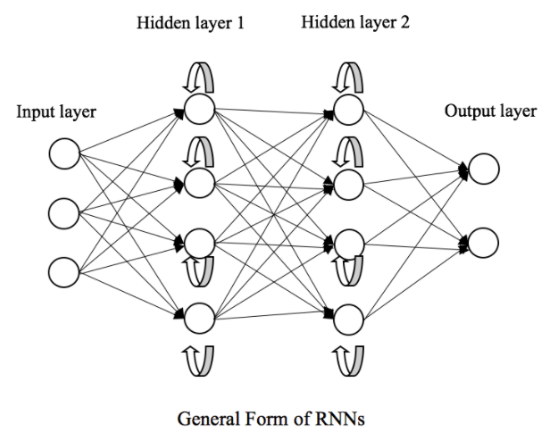
\includegraphics[width=0.47\textwidth]{images/deep_learning/rnn_0.png}}

    \caption{Architecture of a Recurrent Neural Network \cite{Lin20}.}
    \label{fig:dl-1}
\end{figure}

This network is mostly used for natural language processing or data that has a sequential order to it which 
makes an appropriate candidate for learning and detecting software vulnerabilities. 

\subsection{Convolutional Neural Network (CNN)}
\label{sub:convolutional-neural-network}

A Convolutional Neural Network (CNN) is a type of NN that uses convolutional and pooling layers to only 
extract the important parts of a data-point (Figure \ref{fig:dl-2}). The convolutional layers of a CNN outputs a feature map which 
represents important features of the given datum and those feature maps are downsampled with a pooling layer. 
This pooling layer normally comes after a convolutional layer and reduces the complexity of the feature maps. 
Next, the downsampled feature map gets passed to an activation function and then through the output layer of the 
network which would return a vector that represents the final classifications of the given data-point. This final 
vector contains class units each of which are probabilities between 0 and 1. Essentially, one class unit means 
one prediction or classification, two represents two classifications, and so on \cite{Lin20}. There is no 
limit to how many convolutional or pooling layers a CNN can have.

\begin{figure}[h]
    \centering
    \fbox{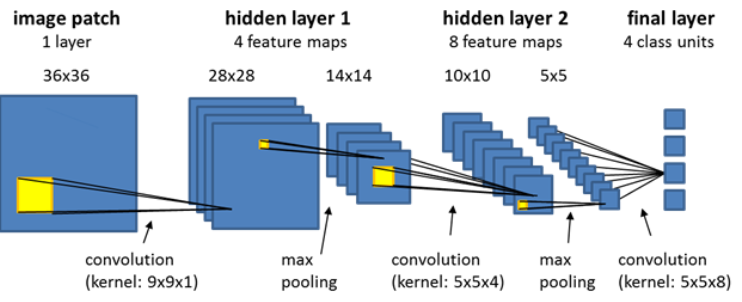
\includegraphics[width=0.47\textwidth]{images/deep_learning/cnn_0.png}}

    \caption{Architecture of a Convolutional Neural Network \cite{Lin20}.}
    \label{fig:dl-2}
\end{figure}

CNNs are primarily used for computer vision tasks such as classification, object detection, and more. 
The most important and relevant attribute for this topic is that CNNs can represent data in the form of 
matrices and properly segment regions of the data (Figure \ref{fig:dl-3}). This is especially useful for when a model needs to segment 
specific blocks of code that are vulnerable to exploits. 

\begin{figure}[h]    
    \centering
    \fbox{
    \begin{tabular}{cc}
        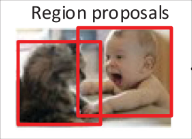
\includegraphics[width=0.26\textwidth]{images/deep_learning/cnn_1.png}
        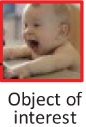
\includegraphics[width=0.13\textwidth]{images/deep_learning/cnn_2.png}
    \end{tabular}
    }
    \caption{Example of image segmentation. A neural network would first segment certain identifiable 
    objects in the picture and then only highlight object of interest \cite{Li22}.}    
    \label{fig:dl-3}
\end{figure}

\subsection{Deep Belief Network (DBN)}
\label{sub:deep-belief-network}

A Deep Belief Network (DBN) is an NN that contains multiple hidden layers of generative models called 
a Restricted Boltzmann Machine (RBM) (Figure \ref{fig:dl-4}). Each RBM in a layer is trainined separately 
from the rest of the layers where the output of each RBM layer is used as input for the next RBM layer until 
it reaches the final output layer of the network.

A Restricted Boltzmann Machine in paticular is a generative model that learns a probability distribution 
of the given input data - this is called a Joint Probability Distribution \cite{Feller57}. Although Figure 
\ref{fig:dl-4} demonstrates that an RBM is a layer, it actually as two addition underlying layers: the 
\textbf{visible} and \textbf{hidden} units. So since the network in Figure \ref{fig:dl-4} has three RBM layers, the 
entire network actually has six additional layers. In the visible layer, the network computes the number 
of visible units, \emph{m}, over the number of hidden units, \emph{n}. Where \emph{v} is the total 
visible units and \emph{h} is the total hidden units (Equation \ref{eq:rbm-0}).

\begin{equation}
\label{eq:rbm-0}
    P(v|h)=\Pi_{i-1}^{m}P(v_{i}|h)
\end{equation}

Conversely, in the hidden layer, the network computes the number of hidden units over the number of 
visible units (Equation \ref{eq:rbm-1}).

\begin{equation}
\label{eq:rbm-1}
    P(h|v)=\Pi_{j-1}^{n}P(h_{j}|v)
\end{equation}

These individual probabilies are then passed through a logistic sigmoid activation function as the final 
output of an RBM layer.

\begin{figure}[h]
    \centering
    \fbox{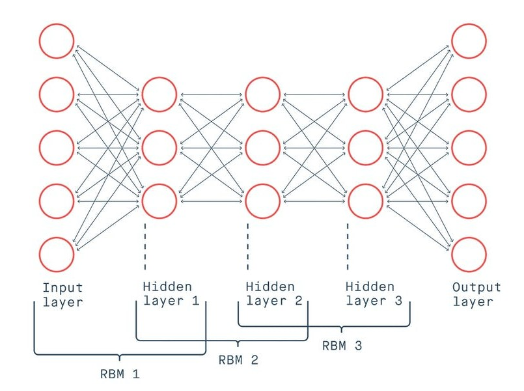
\includegraphics[width=0.47\textwidth]{images/deep_learning/dbn_0.png}}

    \caption{Architecture of a Deep Belief Network \cite{Lin20}.}
    \label{fig:dl-4}
\end{figure}

Data used for networks can be complex in terms of dimensionality, i.e., the datasets that contain software 
vulnerabilities are considered high-dimensional which can slow the performance of a network during training. 
This is a very important unsupervised learning characteristic that makes the DBN an advantageous network 
for this particular problem \cite{Lin20}.






% <><><><><><><><><><><><><><><><><><><>
%          SYSEVR FRAMEWORK - Carter \cite{Li22}
% <><><><><><><><><><><><><><><><><><><>
\section{SySeVR Framework}
\label{sec:sysevr-framework}
SySeVR is the first systematic framework that uses deep learning to detect vulnerabilities in C/C++ source code. The premise of the framework is representing information as vectors which
accomodate both the syntax and semantic information necessary for vulnerability detection. SySeVR uses multiple neural networks to detect various vulnerabilties, using Bidirectional RNNs as its backbone because they are more effective than other neural networks.
In the SySeVR framework, there are the SyVCs and SeVCs components which work together in considering syntax characteristics and semantic information.
\subsection{Syntax-based Vulnerability Candidates (SyVCs)}
\subsection{Semantics-based Vulnerability Candidates (SeVCs)}

\subsection{Method}
\label{sub:method}

\subsection{Results}
\label{sub:results}








\subsection{Limitations}
\label{sub:limitations}
\subsubsection{Narrow Scope}
SySeVR is ultimately designed with a narrow scope, that is, to do vulnerability checks on programs written in
the C or C++ programming language. The dataset of vulnerabilities may be specific to C/C++ issues, thereby requiring
a potential re-imagining of the SySeVR framework so it can become robust and work with multiple languages.
\subsubsection{Limited Characteristics}
The dataset in which SySeVR is trained on to identify vulnerabilities has limited coverage and only focuses on four
kinds of syntax characteristics, covering ~93.6\% of programs in SARD. This dataset is large enough to prove the usability
of SySeVR as a framework, but it is not strong enough to prove this framework can identify vulnerabilities in most real-world
programs. More data will produce a more reliable framework, and this is a focus area for future research.
\subsubsection{Single Model}
This is potentially a large limitation, which forces the question of incorporating more models to flesh out future
vulnerabilities or instead only working with the one. It is quite possible that multiple models will allow more coverage, but
may be far more complicated.
\subsubsection{Robustness}
Given the way SySeVR tests for vulnerabilities, presently it is only possible for the framework to recognize which
block or lines of code the vulnerability exists in. It will be far more useful and robust if the framework is able to
determine the specific line of code, given the semantic relationship that line has with its neighbors. Of course, this is
a focus area for future research.

% <><><><><><><><><><><><><><><><><><><>
%         ADDITIONAL FRAMEWORKS
% <><><><><><><><><><><><><><><><><><><>
\section{Additional Frameworks}
\label{sec:additional-frameworks}

We covered SySeVR in detail because we wanted to introduce what a workflow for detecting vulnerable 
software would look like. However, this process in particular only represents a single piece of something 
much bigger. Ever since the inception of GitHub and open-source software, many new deep learning frameworks have been 
created to analyze many different programming languages and software for vulnerabilities. In this section, 
we are going to provide some insight on some of those frameworks that continue to aid companies and cybersecurity engineers 
when developing software.

\begin{figure*}[h!]
    \centering
    \fbox{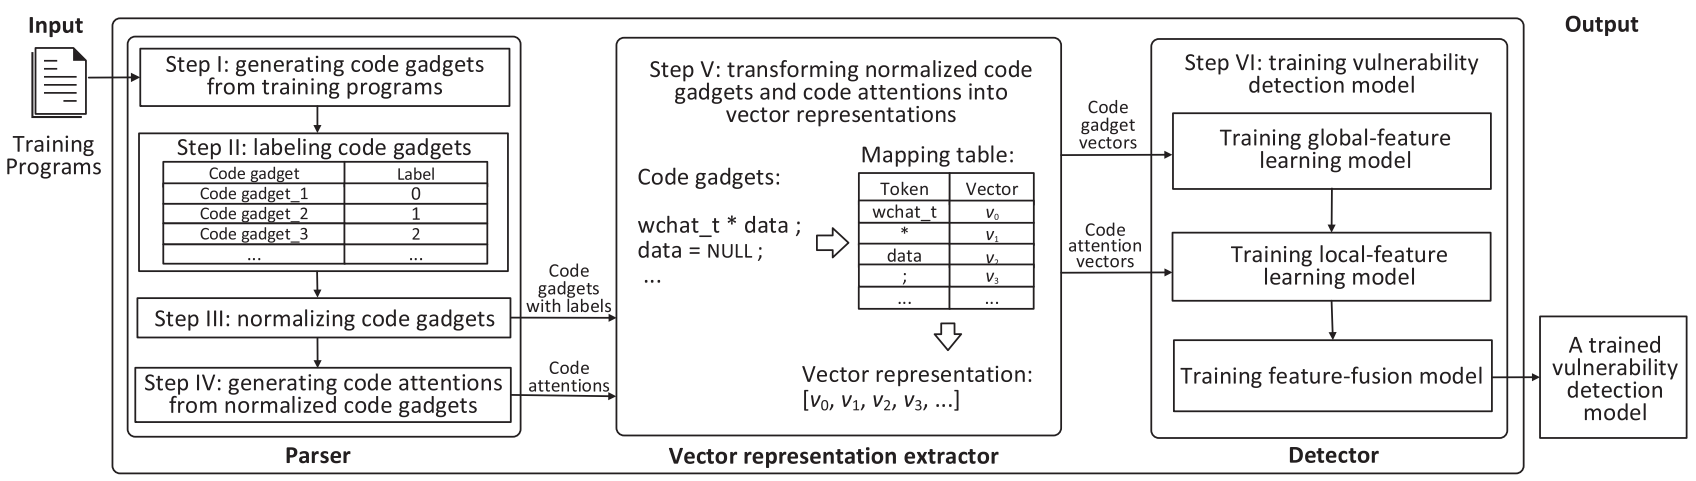
\includegraphics[width=1.0\textwidth]{images/additional_frameworks/vul_dee_pecker_0.png}}

    \caption{Training phase of the VulDeePecker framework \cite{Zou21}.}
    \label{fig:af-0}
\end{figure*}

\begin{figure*}[h!]
    \centering
    \fbox{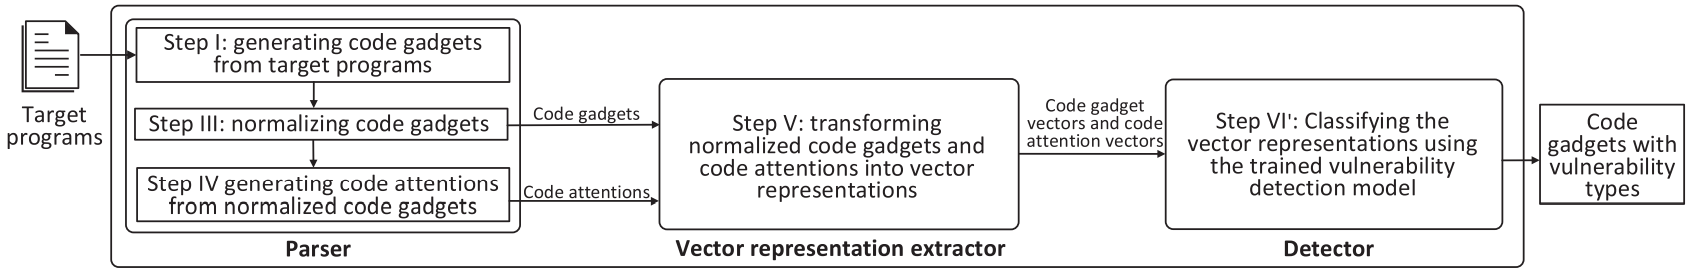
\includegraphics[width=1.0\textwidth]{images/additional_frameworks/vul_dee_pecker_1.png}}

    \caption{Detection phase of the VulDeePecker framework \cite{Zou21}.}
    \label{fig:af-1}
\end{figure*}

% Stefan
\subsection{VulDeePecker: A Deep Learning-Based System for Multiclass Vulnerability Detection}
\label{sub:vuledeepecker}

Some existing frameworks such as SySeVR can only detect the presence of vulnerabilities. However, these 
frameworks cannot pinpoint the types of vulnerabilities that are present in a given source code. This 
section introduces a new deep learning framework callled VulDeePecker which is model that is meant for 
multiclass vulnerability detection \cite{Zou21}.  VulDeePecker stands for Multiclass Vulnerability Deep Pecker.
Multiclass means multiple class labels in deep learning, i.e., the ability to specify how the object of interest 
should be labelled.

The authors of this framework did not use any third party databases such as NVD \cite{Nist00,Zou21}. Instead, 
they created their dataset from scratch and used to train and evaluate their framework. Similar to SySeVR, 
there are two phases defined for VulDeePecker: training and detection. In both phases, there are three major
components: parser, vector representation extractor, and detector (Figures \ref{fig:af-0} and \ref{fig:af-1}). 
Given a sample program, the first component, parser, is responsible for parsing the source code into code gadgets. 
Code gadgets represents the number of code statements that semantically related \cite{Zou21}. The parser would then 
label each code gadget and normalize them based on the total number of gadgets found. With the normalize gadgets, 
the parser would output code attentions which is how we differentiate between each gadget. Along with the attentions,
the gadgets themselves are provided to the extractor. The vector representation extractor essentially transforms the 
gadgets and attention into quantifiable vectors for the learning model called the Detector. 

\begin{figure}[h]
    \centering
    \fbox{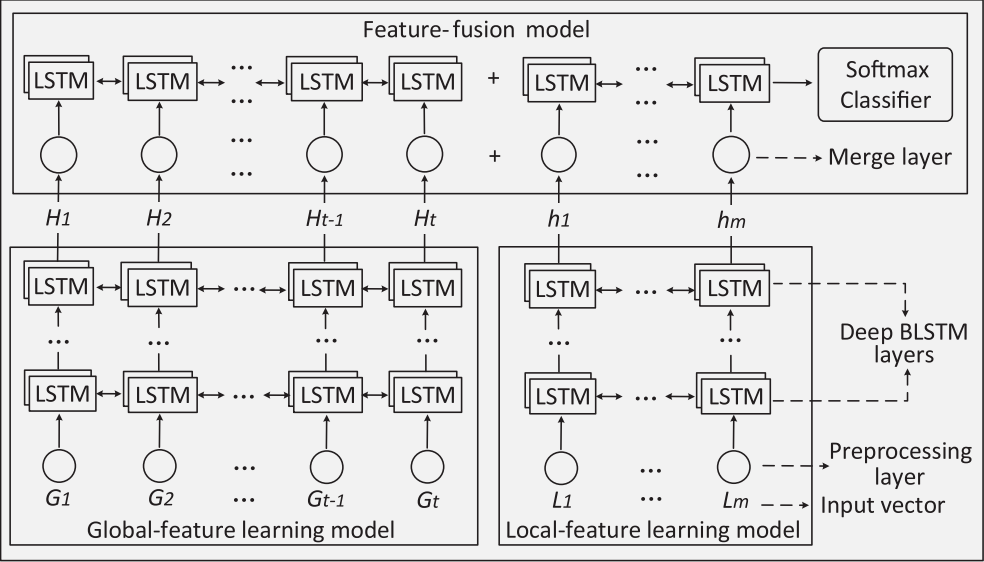
\includegraphics[width=0.5\textwidth]{images/additional_frameworks/vul_dee_pecker_2.png}}

    \caption{Architecture for the BLSTM neural network. \cite{Zou21}.}
    \label{fig:af-2}
\end{figure}

The main detector for this is called the Bidirectional Long-Short Time Memory neural network or BLSTM. It 
is a new type of network that is broken up into three models: feature-fusion, global-feature, and local-feature 
models (Figure \ref{fig:af-2}). In this final step the network can either train with these inputs or make 
a final classification. The detection phase is similar to the training phase, but skips step 2 in the parser 
(Figure \ref{fig:af-1}). 

After training and validation, the VulDeePecker framework was able to achieve false-positive rate of 
0.02\%, false-negative rate of 5.73\%, and an F1 score of 94.69\%. Despite this new state-in-art scores, 
the computational cost significantly increased compared to other existing frameworks.

% Carter \cite{Russell18}
\subsection{Automated Vulnerability Detection Machine Using Deep Representation Learning}
\label{sub:automated-vulnerability-detection-machine-using-deep-representation-learning}

\subsubsection{Strength in Data}
Deep representation learning provides a strong model to detect vulnerabilities using machine learning. Aside from the model
itself, the strength comes from the collection of data available to train the model with. The researchers combined various
sources of data to make a dataset composed of millions of functional-level examples of C/C++ code. Data is at the
functional-level as to keep it the lowest level of granularity while still capturing the flow of subroutines \cite{Russell18}.

Data was sourced from SATE IV (Juliet Test Suite), Debian packages, and public Git repositories to simulate real-world data
for the machine learning model. There are three separate phases to procuring the data inside this immense dataset.

In phase 1, the researchers created their own C/C++ lexer to capture the relevant meaning of certain tokens, but keeping it
generic and small in size. The purpose of this is lexer is to standardize the data inside different code bases, empowering a transfer of learning throughout the dataset.
In phase 2, any duplicated code or code with neglible differences from other samples of code is strictly removed
In phase 3, open-source analyzers Clang, Cppcheck, and Flawfinder were used to generate labels on vulnerable code and what kind of code
errors they are.
Efficient handling of large amounts of data will in turn produce a powerful model capable of using deep representation learning.

\subsubsection{Architecture}
To create vulnerability detection using Deep Representation Learning, the researchers' approach is to combine
neural feature representations of the C/C++ source code with an ensemble classifier known as random forest. In creating
the neural network classifier, the researchers took inspiration from natural language processing. In addition, they take
inspiration from CNNs and RNNs by leveraging feature-extraction similiar to that of sentence sentiment classification.

There are five total stages in the architecture for deep representation learning. Figure \ref{fig:af-3} demonstrates these
five stages, starting with an embedding of the lexer tokens, and ending with random forest classification.

[Pretend Figure \ref{fig:af-3} is here.]
\linebreak
Tokens produced from the lexer are embedded into a fixed k-dimensional representation based on randomly initialized learned embeddings.
In the second stage, feature extraction, both convolutional and recurrent feature extraction approaches were used.
In the third stage, pooling, the results from either convolutional or recurrent features are maxpooled across the sequence length in order to
keep a fixed-size representation.
In the fourth stage, dense layers, there exist two layers of classifying, boosting the classification performance.
In the fifth and final stage, the training data was standardized with similar variables, and any sensitive parameters were tuned using Matthews Correlation Coefficient.
At this stage, selection of models is based on the highest validation from this coefficient.

This model is designed to be robust and have excellent classification performance. The researchers opted to use the
neural features from the pooling stage and use them as inputs to an ensemble classifier like random forest, which in turn
proved to yield very good results. This approach is robust because it allows retraining on new sets of features.

\subsubsection{Results}
In the end, it is evident that the CNN models performed better than the other models. These CNN models were also the fastest to train
and do so with fewer parameters. However, the models using the random forest classifer performed slightly better than the models without random forest classification.
Of the models discussed in this section, CNN + RF performs the best, and further results are tested based on the CNN + RF model.

\begin{figure}[h]
    \centering
    \fbox{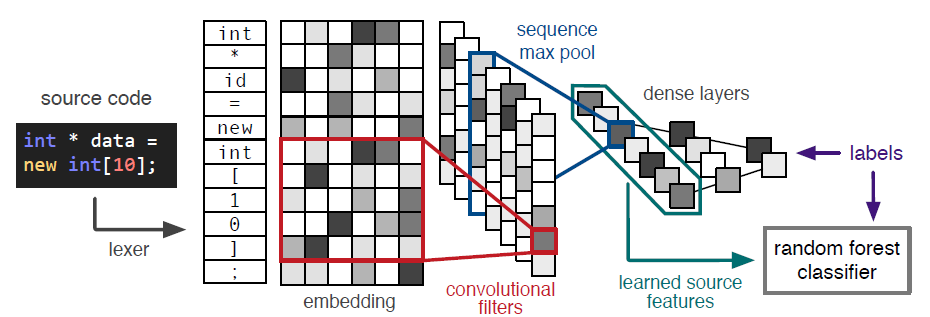
\includegraphics[width=0.47\textwidth]{images/additional_frameworks/deep_repre_learning_1.png}}
    \caption{Convolutional feature activation map. \cite{Russell18}.}
    \label{fig:af-3}
\end{figure}

% Carter 
\subsection{VulDeBERT: A Vulnerability Detection System Using BERT}
\label{sub:vuldebert}
VulDeBERT is another software vulnerability detection system which uses machine learning to detect issues with C/C++ code gadgets. The system stands for Bidirectional Encoder Representations from Transformers (BERT).
In full, the name VulDeBERT is a combination of VulDeePecker and BERT. The significance of VulDeePecker in this section is that it is considered the state-of-the-art detection system, which
VulDeBERT is trying to overcome in terms of detection accuracy \cite{Kim22}. In this section, we will cover three core parts of VulDeBERT, starting with its architecture,
then moving onto its code gadget generation, and finally evaluating its results and seeing how this system compares with the aforementioned VulDeePecker system.
\subsection{Architecture of VulDeBERT}
Similarly to VulDeePecker, VulDeBERT's architecture is made up of two phases; training phase and detection phase.
In the training phase, once VulDeBERT has generated the code gadgets, it will embed these code gadgets into a BERT input representation so that it can train
as a BERT model. The BERT model has its parameters fine-tuned and trained to detect target vulnerabilities. The output from this phase
is sent to a classifer to detect specific vulnerabilities.

The second phase, detection phase, is rather similar to the training phase. However, the code gadget generation does not perform until completion. Instead,
the step in which ambiguous code gadgets are removed does not perform, thereby keeping ambiguous code in the mix of code gadgets.
A vector is produced, containing the source code's gadgets, and rather any vulnerabilities detected in this phase will report the location inside
the vector, otherwise classifying the given vector as safe.

\subsubsection{Code Gadget Generation}
A critical component to VulDeBERT, the researchers for this model developed a new code gadget generation tool to
make sure the inputs into the model is strictly well-structed and semantically related, and wholely extracted from source code files.
As their research is specifically interested in system function calls, the idea is to create a code gadget by collecting
code slices related to a system function call, its caller and its recipient. There are three stages in VulDeBERT's code gadget generation.
To begin, in phase 1, slices are determined to be related to system function calls in some capacity. In phase 2, these slices are
converted into code gadgets. In phase 3, any ambiguous or unclear code gadgets are removed for usability and uniformity. 
Figure \ref{fig:af-4} demonstrates a visualization of this process which may simplify the three phases.

\subsubsection{Evaluating VulDeBERT}
As mentioned at the start, the idea of VulDeBERT is to replace VulDeePecker as a new state-of-the-art vulnerability detection system. Therefore, the evaluation of the system will be
tested against VulDeePecker. As VulDeePecker is not publicly available, the researchers working on VulDeBERT conduct evaluations by remaking the classification model that
VulDeePecker uses, which is the bidirectional LSTM classification model. The recreation of this model shares the same hyperparameters as VulDeePecker.

To account for averages, each evaluation was repeated ten times. The metrics that are to be evaluated are the False Positive Rate, False Negative Rate, True
Positive Rate, Precision, and an F1 score. Out of the tests performed, it is found that VulDeBERT achieved a mean F1 score of ~94.6\% compared to VulDeePecker, which only achieved a score of ~86.6\%. The detection accuracy of VulDeBERT was generally higher than VulDeePecker's accuracy, making the system a promising competitor
to VulDeePecker.

% @stefan it may be nice if this could span the whole width and not overlap other figure(s)
% otherwise it is fine as is
\begin{figure}[h!]
    \centering
    \fbox{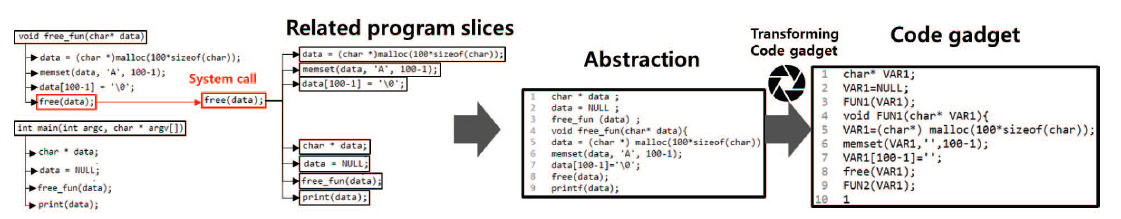
\includegraphics[width=0.5\textwidth]{images/additional_frameworks/vul_de_bert_1.png}}
    \caption{Three phases of Code Gadget generation. \cite{Kim22}.}
    \label{fig:af-4}
\end{figure}


% <><><><><><><><><><><><><><><><><><><>
%         FUTURE WORK - Stefan
% <><><><><><><><><><><><><><><><><><><>
\section{Future Work}
\label{sec:future-work}

As for future work, these open-source deep learning frameworks can and should be imbedded into existing 
development practices such as version control and continuous integration/delivery pipelines.

\subsection{Integration with Version Control}
\label{sub:integrating-with-version-control}

Version control is one of most popular practices in the software industry it allows engineers to keep track 
of changes and to collaborate with others in the most efficient way possible. 

Existing version control systems such as Git \cite{Torvalds05} and GitHub \cite{Werner08} should start leveraging these vulnerability 
detection systems to analyze committed code so that it can detect bugs or vulnerabilities as fast as 
possible. This would help engineers quickly understand their flaw and fix them before it even hits production.
Thus, minimizing the risk of attackers exploiting those vulnerabilities.

\subsection{Integrating with CI/CD Pipelines}
\label{sub:integrating-with-cicd-pipelines}

Another late addition to the software development cycle is continuous integration/delivery (CI/CD). 
CI/CD is an approach that utilizess automation to frequently release audited code changes to production. 
Whenever code is pushed to the main production branch, it triggers an event that performs integration 
testing and validation. If it fails testing, then it does not get push to production. Otherwise, it is 
released. This process is called a pipeline and existing vulernability detection systems should be integrated 
with this CI/CD pipeline. Pushed software that passes testing can still contain vulneribilities and adding 
that layer to the pipeline would further prevent these vulnerabilities from getting released where attackers 
reside.

% <><><><><><><><><><><><><><><><><><><>
%          CONCLUSION - Carter
% <><><><><><><><><><><><><><><><><><><>
\section{Conclusion}
\label{sec:conclusion}
[text goes here.]

% <><><><><><><><><><><><><><><><><><><>
%            REFERENCES
% <><><><><><><><><><><><><><><><><><><>
{\small
\bibliographystyle{ieee_fullname}
\bibliography{egbib}
}

\end{document}
